\section{Projection and sampling}
The optional central angular camera uses $r(\theta)=\theta(1+k_1\theta^2+k_2\theta^4+k_3\theta^6+k_4\theta^8)$, with $\theta=\operatorname{atan2}(\sqrt{x^2+y^2},-z)$. Full pixel-space $K$, image dimensions, half-pixel centers, model version, coefficients and calibrated angular domain are exported per view. Monotonicity is certified over the entire domain using interval derivative bounds. The coefficient order matches OpenCV fisheye (Kannala--Brandt), verified against its forward-hemisphere equations; OpenCV integer-centered pixels require subtracting 0.5 from the exported principal point and converting the view basis to right/down/forward. The inverse supports rays behind the optical plane, beyond the domain of OpenCV routines based on the front-hemisphere arctangent. This is a central camera model, not rolling shutter or a non-central lens.

Lens assignment is seeded by scene and camera index before placement retries. Configuration controls its Bernoulli probability, continuous diameter FOV, polynomial variation, anisotropy, principal-point displacement and circular, full-frame/diagonal or explicitly elliptical fit. Circular fits enforce equal focal axes and a contained disk; elliptical fits contain the sampled ellipse; diagonal fits cover every sensor corner, including principal-point shifts. The audited lens program uses probability 0.5, a 140--210 degree diameter range and 0.2 circular probability. In 1,024 consecutive seeds with 12 slots each, 6066 of 12288 assignments are angular and 1223 of those are circular. Calibration validation and exact replay pass for every assignment. The admitted pose distribution is affected by obstacle and shared-surface constraints; lens assignment is preserved. Camera motion and baseline controls remain independent.

\section{Rendering and annotation contract}
Up to five co-located perspective faces retain the PBR renderer, shadows, lighting and exposure. Guard bands and a GPU angular resolve produce the final image; faces are implementation details and consume no dataset camera indices. SSAA averages RGB in linear light. Final-pixel-center rays independently intersect authoritative annotation triangles in a shared BVH. Fisheye depth is positive ray range; pinhole depth remains positive axial depth. Invalid lens pixels and surface misses are distinct through the calibrated domain mask. Normals are expressed in the logical camera frame; semantic IDs are never interpolated. Glass follows the selected geometric surface policy, not a refracted or reflected RGB light path.

Forward flow traces the preceding capture's surface and projects its corresponding point at the next controlled timestamp. Co-visibility projects each source surface through the target model and tests symmetric tangent-plane agreement at the nearest target pixel. Finite sampling can leave small holes at thin silhouettes; this is the existing dataset visibility policy. Mixed lenses and circular validity use the same projection contract. Only logical cameras contribute bits to the additive membership mask. Burn and Python tensor archives use a versioned mixed-lens contract with per-view model identifiers and five angular parameters; pinhole-only archives preserve version 1. Direct GPU transports retain the same per-view metadata and on-device color conversion.

\section{Bounded qualification}
The analytic fixture uses a moving occluder, two angular cameras and one pinhole camera over three synchronized captures, with unrelated render updates between captures. Maximum position error is 0.0037 mm; maximum forward-flow error is 0.000123 pixels across 36471 correspondences. There are 63661 co-visibility comparisons away from silhouette discontinuities and 0 mismatches. These tests exercise occlusion, rearward rays, optical-center displacement and anisotropy.

The furnished-room cohort contains 6 consecutive rooms, three cameras and two timestamps at $512\times512$, with automatic $2\times$ SSAA and full scene quality. All 36 captures pass self-reprojection (maximum 0.000407 pixels) and unit-normal checks. The realized diameter range is 153.0--209.8 degrees. Figures show actual, uncorrected renderer output; dim and bright scenes remain in the gallery. Geometry and lens settings, calibration, software provenance and artifact checksums accompany every record.

\begin{figure}[ht]\centering
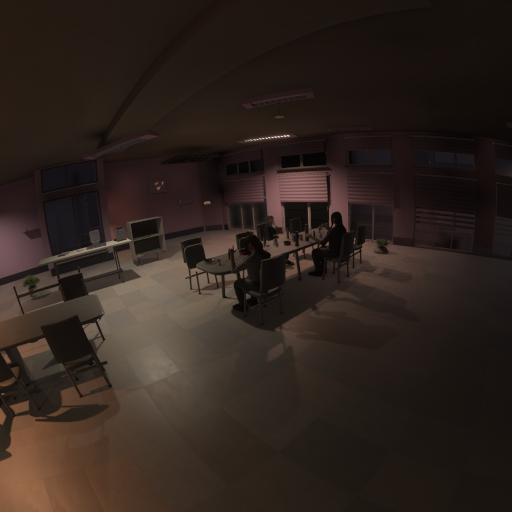
\includegraphics[width=.32\linewidth]{room_401_view_0.png}
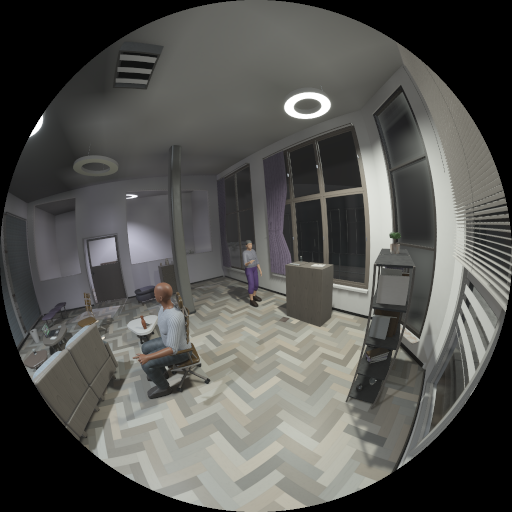
\includegraphics[width=.32\linewidth]{room_402_view_1.png}
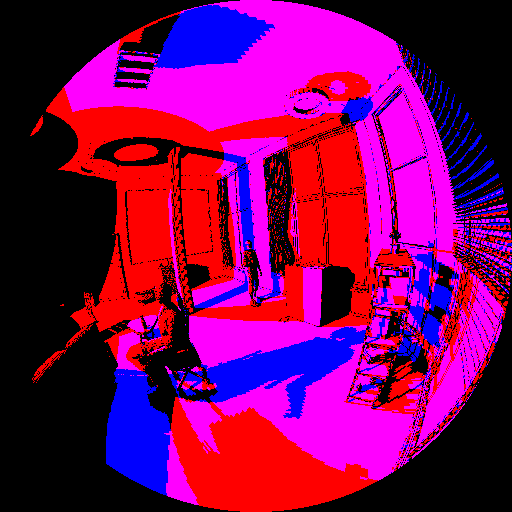
\includegraphics[width=.32\linewidth]{room_402_view_1_co_visibility.png}
\caption{Diagonal and circular fisheye RGB; additive co-visibility from the same circular view (camera 1). Red: camera 0; blue: camera 2; magenta: both; black: no shared peer or invalid lens domain. The full gallery includes all rooms and aligned annotations.}\end{figure}

\section{Throughput and limits}
On the recorded adapter \texttt{llvmpipe (LLVM 20.1.2, 256 bits) (Vulkan)} (no concurrent training launched by this capture command), the completed-generation rate excluding the first room was 0.010 rooms/s or 0.058 camera/time images/s. The first room took 103.267 seconds and is reported separately. Application startup and PNG/JSON report writing are excluded; rendering, scene work and capture readback are included. These are bounded observations of the recorded workload, not a memory-stability guarantee. Five perspective faces cost more than a single pinhole image; shared scene assets/BVH, indexed-vertex transforms, compact BVH partitioning, nearest-first traversal, stable geometry reuse, and the capture activity gate bound redundant work. The disabled path creates no angular textures or BVH.

Measurements use the build recorded in the capture protocol, 256 diffuse-GI rays, GPU material synthesis, furnishing density 0.65 and human density 0.25. Other host workloads are uncontrolled. Software adapters measure software rendering and must not be interpreted as hardware GPU training throughput. Browser/Metal runtime and cross-vendor performance require separate qualification.

Screen-space effects remain face-local; the guarded color resolve is not a path tracer. RGB uses perspective-face clipping while exact geometric targets use the calibrated ray range. Geometry within the configured operating range is the qualification domain; grazing near/far boundary behavior, arbitrary optical systems, hardware-vendor parity and downstream learning gains require further qualification. The main architectural cohort and lens addendum each carry their capture provenance.

\subsection{Photometric face-boundary qualification}
Identical world rays are compared across all eight adjacent face pairs at fixed exposure, with a continuous environment map. Ambient, shadowed directional, point and spot cases vary the direct illumination while retaining the emissive object and bloom; the combined case also includes SSAO. Glass transmission and metallic reflection are present throughout. Per-boundary and aggregate thresholds are checked. These measurements test raster consistency, not physical accuracy against a path tracer.
\begin{center}\begin{tabular}{lrrr}\toprule
Case & Mean error & 95th percentile & Maximum \\
\midrule
ambient & 0.00420 & 0.02233 & 0.04583 \\
directional & 0.00716 & 0.03082 & 0.05379 \\
point & 0.00384 & 0.02074 & 0.04431 \\
spot & 0.00329 & 0.02049 & 0.04401 \\
combined & 0.00157 & 0.00642 & 0.03514 \\
\bottomrule\end{tabular}\end{center}
Errors are maximum-channel absolute differences in tone-mapped linear RGB before the composite. Maximum outliers are retained; screen-space and finite shadow-map approximations are not claimed to be exactly invariant across faces. The final composite blends only the guarded overlap. A separate GPU probe executes the production compositor on these rendered textures, approaching each boundary from either side by $10^{-6}$ radians; every illumination case must have maximum discontinuity below 0.002 and mean below 0.0001. Geometric and categorical targets are not blended.
\paragraph{Remaining photometric limitation.} The raw, pre-composite boundary budget did not pass for every pair. This result is retained as a failed diagnostic, even though all final-composite continuity checks passed. View-local postprocessing can produce different radiance estimates for the same ray; blending removes a hard boundary, but does not establish global photometric invariance or path-traced accuracy.
